\section{Part 2: Application of Model}

To simulate our discrete-time model to real-world scenarios, we need to choose three distinct plots of land from a temperate, arid, and tropical region with relatively low human interference. So, we randomly selected three 
"open" regions in the United States to examine. The regions selected for the temperate, arid, and tropical regions are Clay, New York; Phoenix, Arizona; and Florida Keys; Florida, respectively.

\subsection{Climate Calibration}

To calibrate our model to each selected region, which differs by climate, consumers, and soil nutrition, several \textit{hyperparameters} are necessary, listed below. We use the term hyperparameters to designate global values that are not directly passed into our model but still change the output of the model. 

\begin{itemize}
    \item Temperature — The local temperature, in degrees Fahrenheit, over 2022 will be necessary to compare with a dandelion's optimal range of temperatures for growth.
    \item Light Levels — The local average hours of sunshine over 2022 will be necessary to compare with a dandelion's optimal sunshine range for growth.
    \item Potassium and Nitrogen Levels — Several key factors in determining a climate used in our model include the yearly temperature data, light levels, and Potassium and Nitrogen levels (ppm) in the local soil. Since Potassium levels are closely correlated with soil moisture, we did not choose to calibrate our model with rainfall.    
\end{itemize}

See our code in Appendix 1 for more details. 

\subsection{Regional Results}

\subsubsection{Temperate Region}

To begin, we selected Clay, NY (in Upstate NY) as the region of interest because New York is generally considered as a region of temperate climate.

Next, we obtained data detailing the local temperature, light level, soil composition, and wind data to calibrate the our model's \textit{regional parameters.} Our results for this region are summarized in \ref{fig:temperatespread} where t  time and n represents the number of dandelions. Additionally, the graphs represent the dimensions of the open field we began with. Recall that our first dandelion started at (0,0).

\begin{figure}[h!]
\centering
    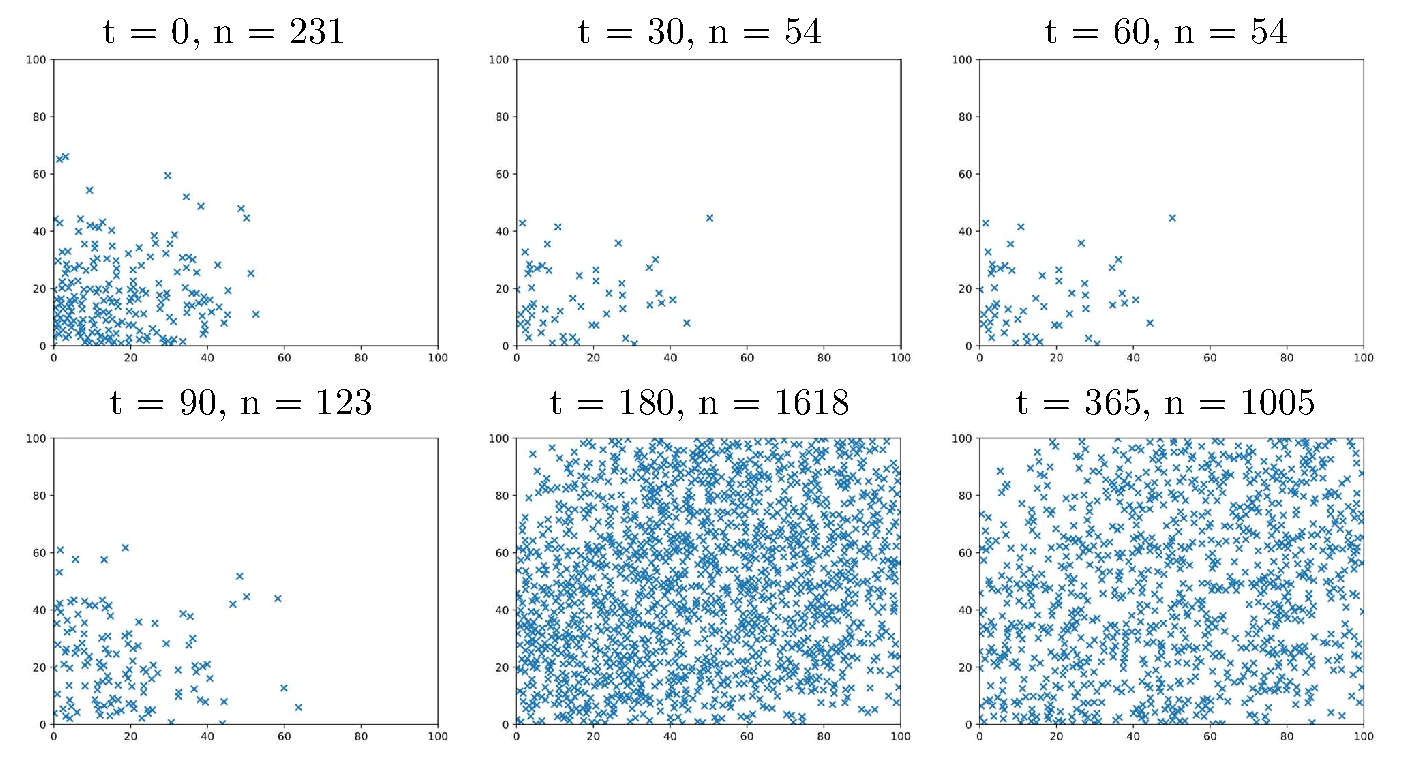
\includegraphics[scale=0.5]{figures/moderateclimatespread.pdf}
    \captionsetup{width=0.9\textwidth}
    \caption{\textbf{From left to right, top to bottom: dandelions spread plot of land over time in Clay, NY.} Each mark labels a spot where a dandelion (either in seed or plant phase) is located at that time stamp in a 100-meter by 100-meter square plot of land.}
    \label{fig:temperatespread}
\end{figure}

As our model initialized the first puffball in the bottom-left corner of the plot of land (Coordinate \((0, 0)\)), one interesting observation is that the stochastic seed dispersal process seems to uniformly cover the plot of land over time. However, it is essential to note that \textit{not all seeds survive} the dispersal process. After 30, 60, and 90 days of simulation from the beginning of the calendar year, the seeds began to disperse farther from the starting point. At the 180-day mark, we see a spike in the number of seeds and dandelion plants due to the effects of optimal climate conditions for a dandelion's blooming phase. After the blooming phase, we see that through day 365 all surviving agents that are left are plants in their dormancy stage.

\begin{figure}[h!]
\centering
    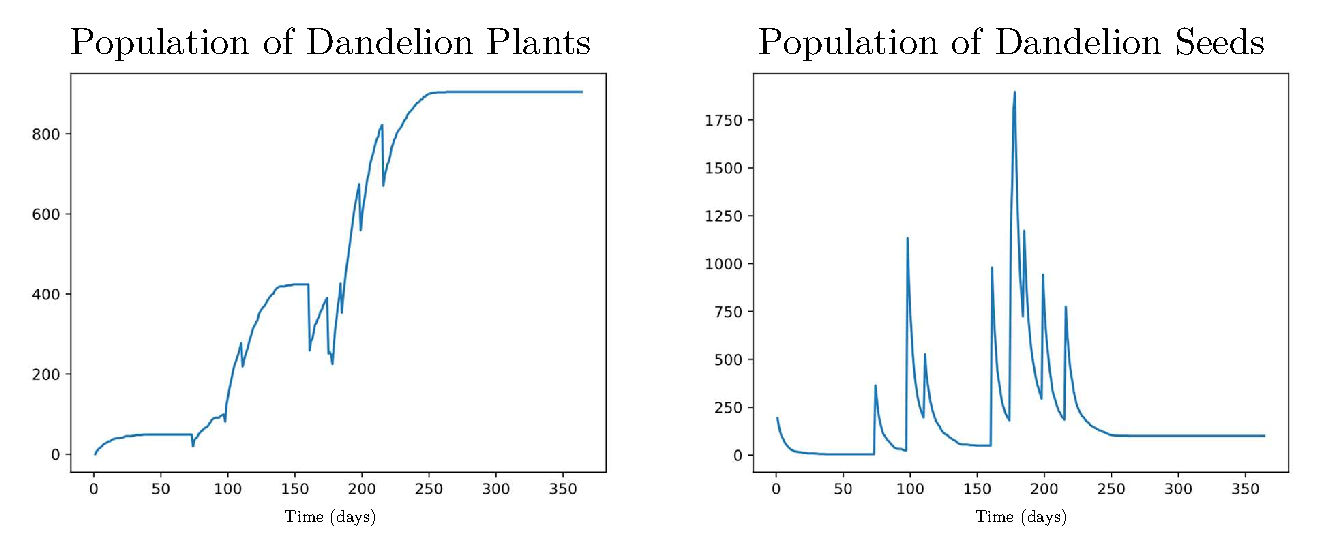
\includegraphics[scale=0.5]{figures/moderateclimatepopulation.pdf}
    \captionsetup{width=0.9\textwidth}
    \caption{\textbf{Growth in population of dandelion plants and seeds over time in Clay, NY.} The simulation began with a single puffball at coordinate \((0, 0)\)}
    \label{fig:temperatepopulation}
\end{figure}

Secondly, a visualization of the growth of dandelion population and seed population over time shows us two key results

\begin{enumerate}
    \item Dandelion plants go through two main blooming processes (spikes in population increase) throughout a year, which is consistent with other findings \cite{noauthor_dandelion_nodate-2}.
    \item Dandelion plant populations remain dormant in winter and fall months while dandelion seeds do not spread much, or at all, in the colder months, which is a unique property of perennial plants (CITE!!!).
\end{enumerate}

\subsubsection{Arid Region}

In Phoenix, Arizona, we obtained new climate and soil nutrition data from several sources (CITE!) We then re-initialized our model with these new hyperparameters and ran our simulated model.

\begin{figure}[h!]
\centering
    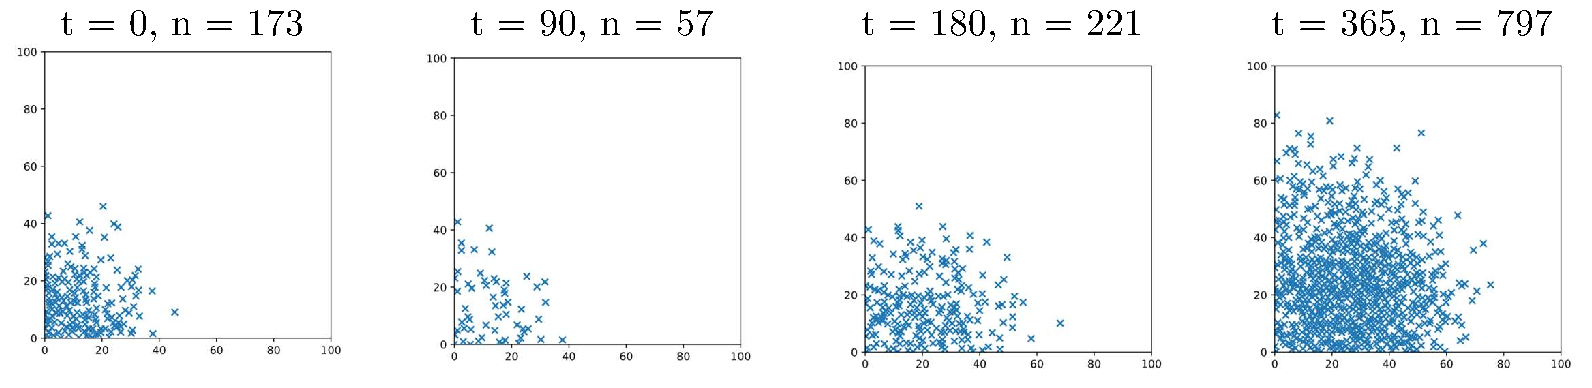
\includegraphics[scale=0.6]{figures/arizonaspread.pdf}
    \captionsetup{width=0.9\textwidth}
    \caption{\textbf{From left to right: dandelions spread plot of land over time in Phoenix, Arizona} Each mark labels a spot where a dandelion (either in seed or plant phase) is located at that time stamp in a 100 meter by 100 meter square plot of land.}
    \label{fig:arizonaspread}
\end{figure}

\begin{figure}[h!]
\centering
    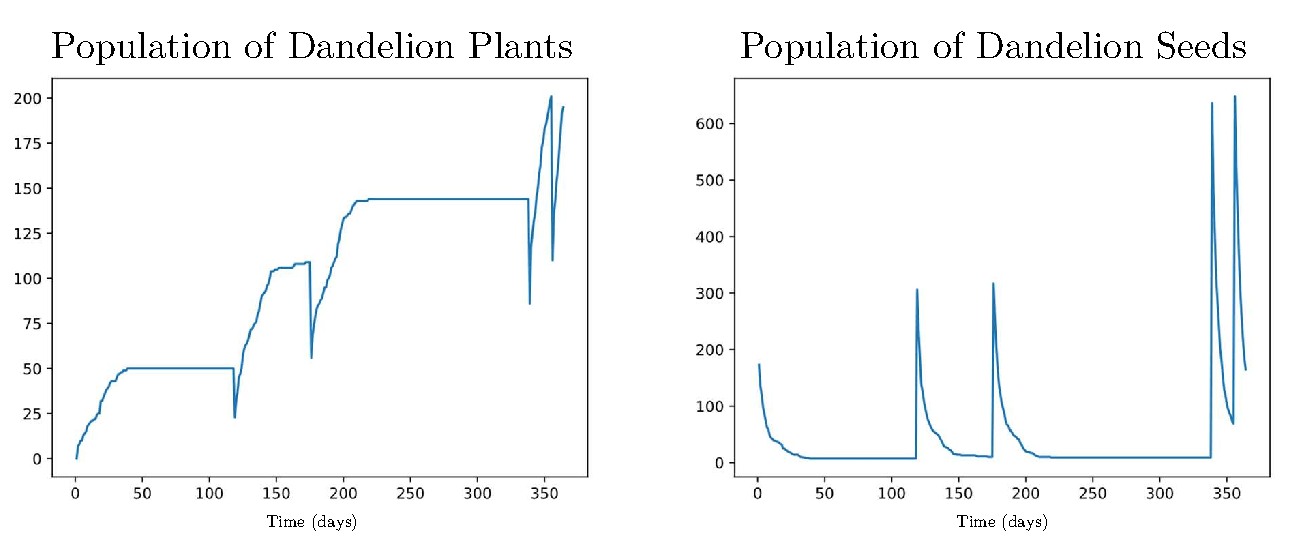
\includegraphics[scale=0.5]{figures/arizonapopulation.pdf}
    \captionsetup{width=0.9\textwidth}
    \caption{\textbf{Dandelion plant population growth in Phoenix, Arizona.}}
    \label{fig:arizonapopulation}
\end{figure}

\subsubsection{Tropical Region}

With calibrating to Florida's Tropical climate in the Florida Keys, we arrived at the following results for the dandelion growth and spread over a period of one year. The calibrated climate data points were pulled from numerous sources as listed (CITE!!!).

One important takeaway of tropical regions is that blooming seasons tend to occur during the winters, when the temperature adheres to the 60 to 70 degree range. Furthermore, we see that dandelion populations remain mostly stagnant over summer months, where the summer heat may take away from dandelion growth.

\begin{figure}[h!]
\centering
    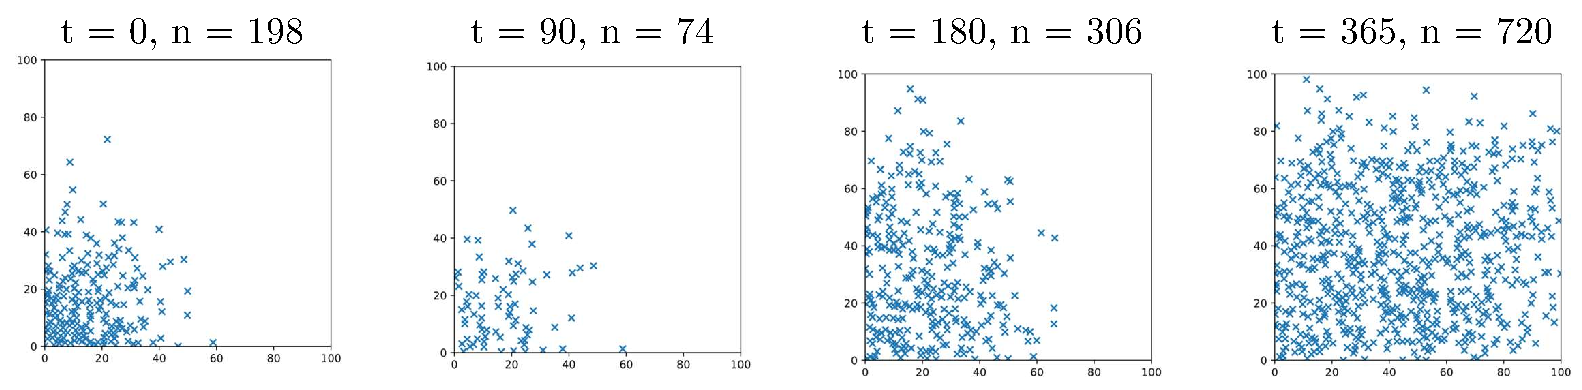
\includegraphics[scale=0.6]{figures/floridadistributions.pdf}
    \captionsetup{width=0.9\textwidth}
    \caption{\textbf{From left to right: dandelions spread plot of land over time in Florida Keys, Florida} Each mark labels a spot where a dandelion (either in seed or plant phase) is located at that time stamp in a 100 meter by 100 meter square plot of land.}
    \label{fig:floridaspread}
\end{figure}

\begin{figure}[h!]
\centering
    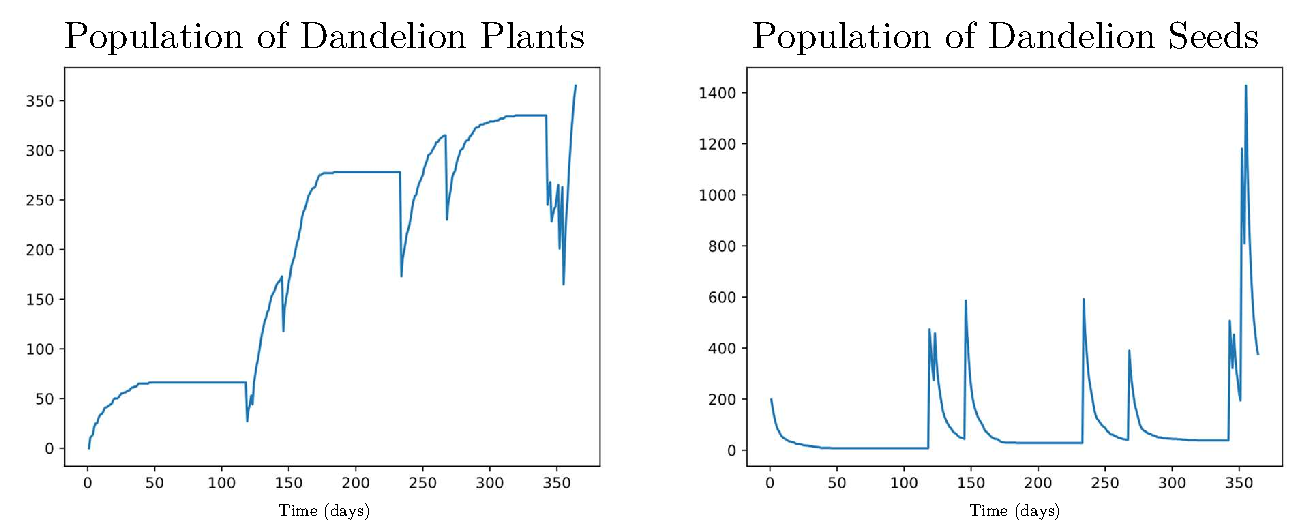
\includegraphics[scale=0.5]{figures/floridapopulation.pdf}
    \captionsetup{width=0.9\textwidth}
    \caption{\textbf{Dandelion plant population growth in Florida Keys, Florida.}}
    \label{fig:floridapopulation}
\end{figure}

We can conclude that from the models applied to the three regions, dandelions follow logistic growth to the most part. We will revisit this idea of logistic growth in the following impact score model.